\section{METODOLOGIA}
\label{sec:metod}

\subsection{Extração de dados sobre produtos}

\cite{alonso2015agente} realizou um estudo sobre extração de preços em sites de \emph{e-commerce}. Neste trabalho foi desenvolvido um agente de \emph{Shopping Comparison} que utilizava padrões em documentos HTML para obter produtos e seus respectivos atributos.Porém este estudo possuía o ponto deficiente de não conseguir obter informações de \emph{websites} que utilizam a linguagem Javascript para exibir o preços dos produtos assincronamente, o que é uma prática comum em sites atuais.

O presente trabalho tratará os pontos deficientes do estudo de \citeonline{alonso2015agente}, e também abordara outras funcionalidades da aplicação em si.

Um dos recursos do sistema proposto é proporcionar a comparação de preços de peças de computador entre diversas lojas de \emph{e-commerce}, para se obter a informação de cada peça com seus respectivos preços e vendedores o sistema utilizara de um algoritmo de extração de dados. Tal algoritmo sera desenvolvido em Javascript e será executado utilizando o PhantomJS.
Os dados que deveram ser extraídos dos \emph{websites} voltados para o \emph{e-commerce} são:


\begin{itemize}
\setlength{\itemsep}{-0.3ex}
\item nome do produto.
\item link da imagem do produto.
\item preço do produto.
\item descrição do produto.
\item link para a compra do produto.
\end{itemize}


As informações do produto como nome, \emph{link} da imagem, preço, \emph{link} para a compra serão necessárias para identificar o produto, exibir sua imagem e manter informações sobre o vendedor.

Para se obter tais informações será criado um \emph{script} que adotara a seguinte estratégia: obter a árvore DOM do \emph{website} utilizando funções disponibilizadas pelo phatomJS e ai então utilizando a DOM juntamente com seletores CSS o algoritmo ira buscar pelo carácter \$ pois o mesmo denota preço, ao encontra-lo  analisara os elementos próximos do mesmo nível em busca de uma imagem e nome do produto. Se tais elementos forem localizados, o algoritmo então conseguiu identificar um possível produto.Para confirmar que o item obtido é o que se procura, o algoritmo ira \"subir\" alguns níveis na arvore DOM e então procurar nos elementos próximos por itens semelhantes, se uma sequência de produtos semelhantes forem encontrados, o algoritmo então ira armazenar estes itens em uma lista e os enviara para a aplicação.


\subsection{Persistência dos dados}

O sistema proposto possuirá 2 tabelas essenciais no banco de dados, sendo a primeira de lojas, que conterá informações sobre as lojas de \emph{e-commerce}, a segunda tabela contará com informações sobre os produtos e será preenchida com os dados obtidos por meio do algoritmo de extração de dados, tais dados serão tratados e terão sua integridade testada antes de serem salvos.

\begin{figure}[!h!t!b]
\centering
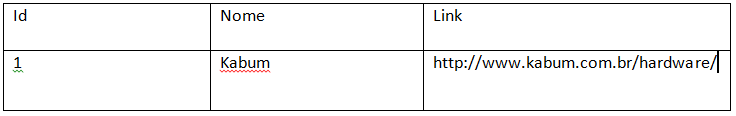
\includegraphics[width=\columnwidth]{img/imagem8-tcc}
\caption{Exemplo de uma tabela de lojas do banco de dados.}
\end{figure}



\begin{figure}[!h!t!b]
\centering
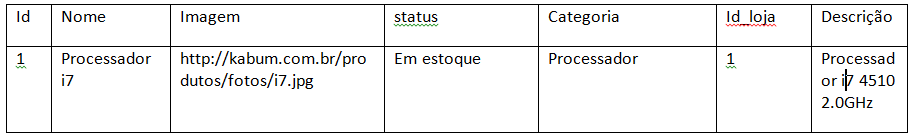
\includegraphics[width=\columnwidth]{img/imagem9-tcc}
\caption{Exemplo de uma tabela de produtos de um banco de dados.}
\end{figure}

A figura~7 representa uma tabela de lojas no banco de dados, tal tabela conterá o nome,\emph{link} para o site da loja e id de cada empresa que terá seus dados extraídos.

A figura~8 representa uma tabela de produtos no banco de dados, esta tabela ira conter informações como: id,nome,imagem,status,categoria,descrição e um identificador que informara a qual loja este produto pertence.


\subsection{Listagem de produtos com comparação de preços}

Com os dados extraídos de diferentes lojas de \emph{e-commerce} voltadas para o comércio de hardware, sera possível a implementação de uma interface \emph{web} que auxilie ao usuário na montagem do próprio computador personalizado. tal interface sera implementada utilizando-se as linguagens HTML,Javascript e CSS. 


Nela o usuário terá acesso a diferentes tipos de peças de computadores o sistema destacara a peça mais barata de cada categoria e seu respectivo vendedor.


